\clearpage
\section{Phân hệ Danh mục Sản phẩm (Product Catalog)}

\subsection{Đặc tả Use Case}
Phân hệ Danh mục Sản phẩm cho phép người dùng khám phá toàn bộ thực đơn của BrewLite, tìm kiếm đồ uống theo tên và lọc theo các phân loại như Cà phê hoặc Trà. Sơ đồ Use Case được biểu diễn tại Hình~\ref{fig:usecase-product-catalog}.

\begin{figure}[H]
    \centering
    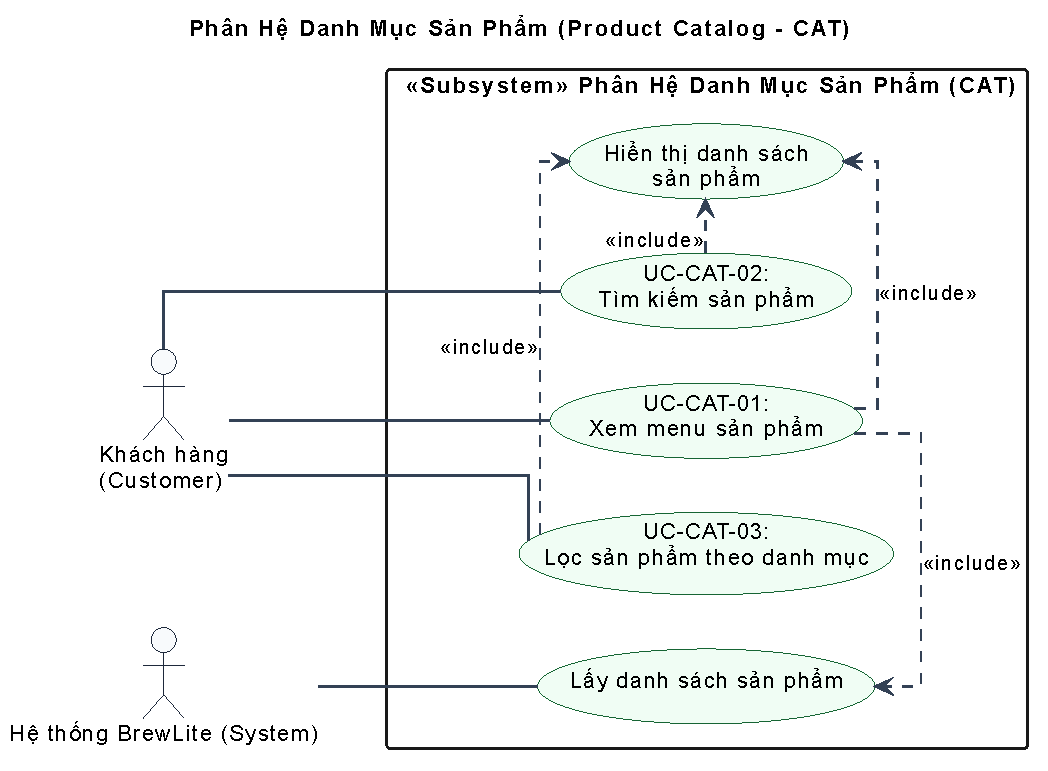
\includegraphics[width=0.75\textwidth]{figures/usecase-product-catalog.pdf}
    \caption{Sơ đồ Use Case - Phân hệ Danh mục Sản phẩm}
    \label{fig:usecase-product-catalog}
\end{figure}

\begin{table}[H]
\centering
\small
\caption{Đặc tả Use Case: Xem và Tìm kiếm Danh mục Sản phẩm (UC-CAT-01)}
\label{tab:uc-spec-catalog}
\begin{tabularx}{\textwidth}{p{2.8cm}X}
\toprule
\textbf{Mục} & \textbf{Chi tiết Đặc tả} \\
\midrule
\textbf{Actor} & Khách vãng lai, Khách hàng đăng nhập \\
\midrule
\textbf{Tiền điều kiện} & Hệ thống có dữ liệu sản phẩm và danh mục đã được kích hoạt trong CSDL. \\
\midrule
\textbf{Hậu điều kiện} & Danh sách sản phẩm tương ứng hiển thị trực quan trên giao diện thực đơn. \\
\midrule
\textbf{Luồng chính} & 
1. Người dùng truy cập trang Thực đơn (\texttt{/products}).\newline
2. Giao diện gửi request \texttt{GET /api/v1/categories} và \texttt{GET /api/v1/products}.\newline
3. Hệ thống trả về danh sách danh mục (Cà phê, Trà) và danh sách 10 sản phẩm (6 món cà phê, 4 món trà theo seed data).\newline
4. Khách hàng nhấp chọn tab phân loại (ví dụ "Cà phê") hoặc nhập từ khóa tìm kiếm (ví dụ "Latte").\newline
5. Hook \texttt{useProductCatalog} lọc lại danh sách hiển thị tương ứng kèm nhãn giá cơ bản và trạng thái còn hàng/hết hàng. \\
\midrule
\textbf{Luồng ngoại lệ} & 
- Lỗi kết nối mạng hoặc máy chủ backend: Hiển thị thông báo tải dữ liệu thất bại và cung cấp nút thử lại.\newline
- Không tìm thấy sản phẩm phù hợp: Hiển thị thông báo "Không tìm thấy sản phẩm nào phù hợp". \\
\bottomrule
\end{tabularx}
\end{table}

\clearpage
\subsection{Sơ đồ Hoạt động (Activity Diagram)}
Quy trình nạp và lọc danh mục sản phẩm được mô tả tại Hình~\ref{fig:activity-product-catalog}.

\begin{figure}[H]
    \centering
    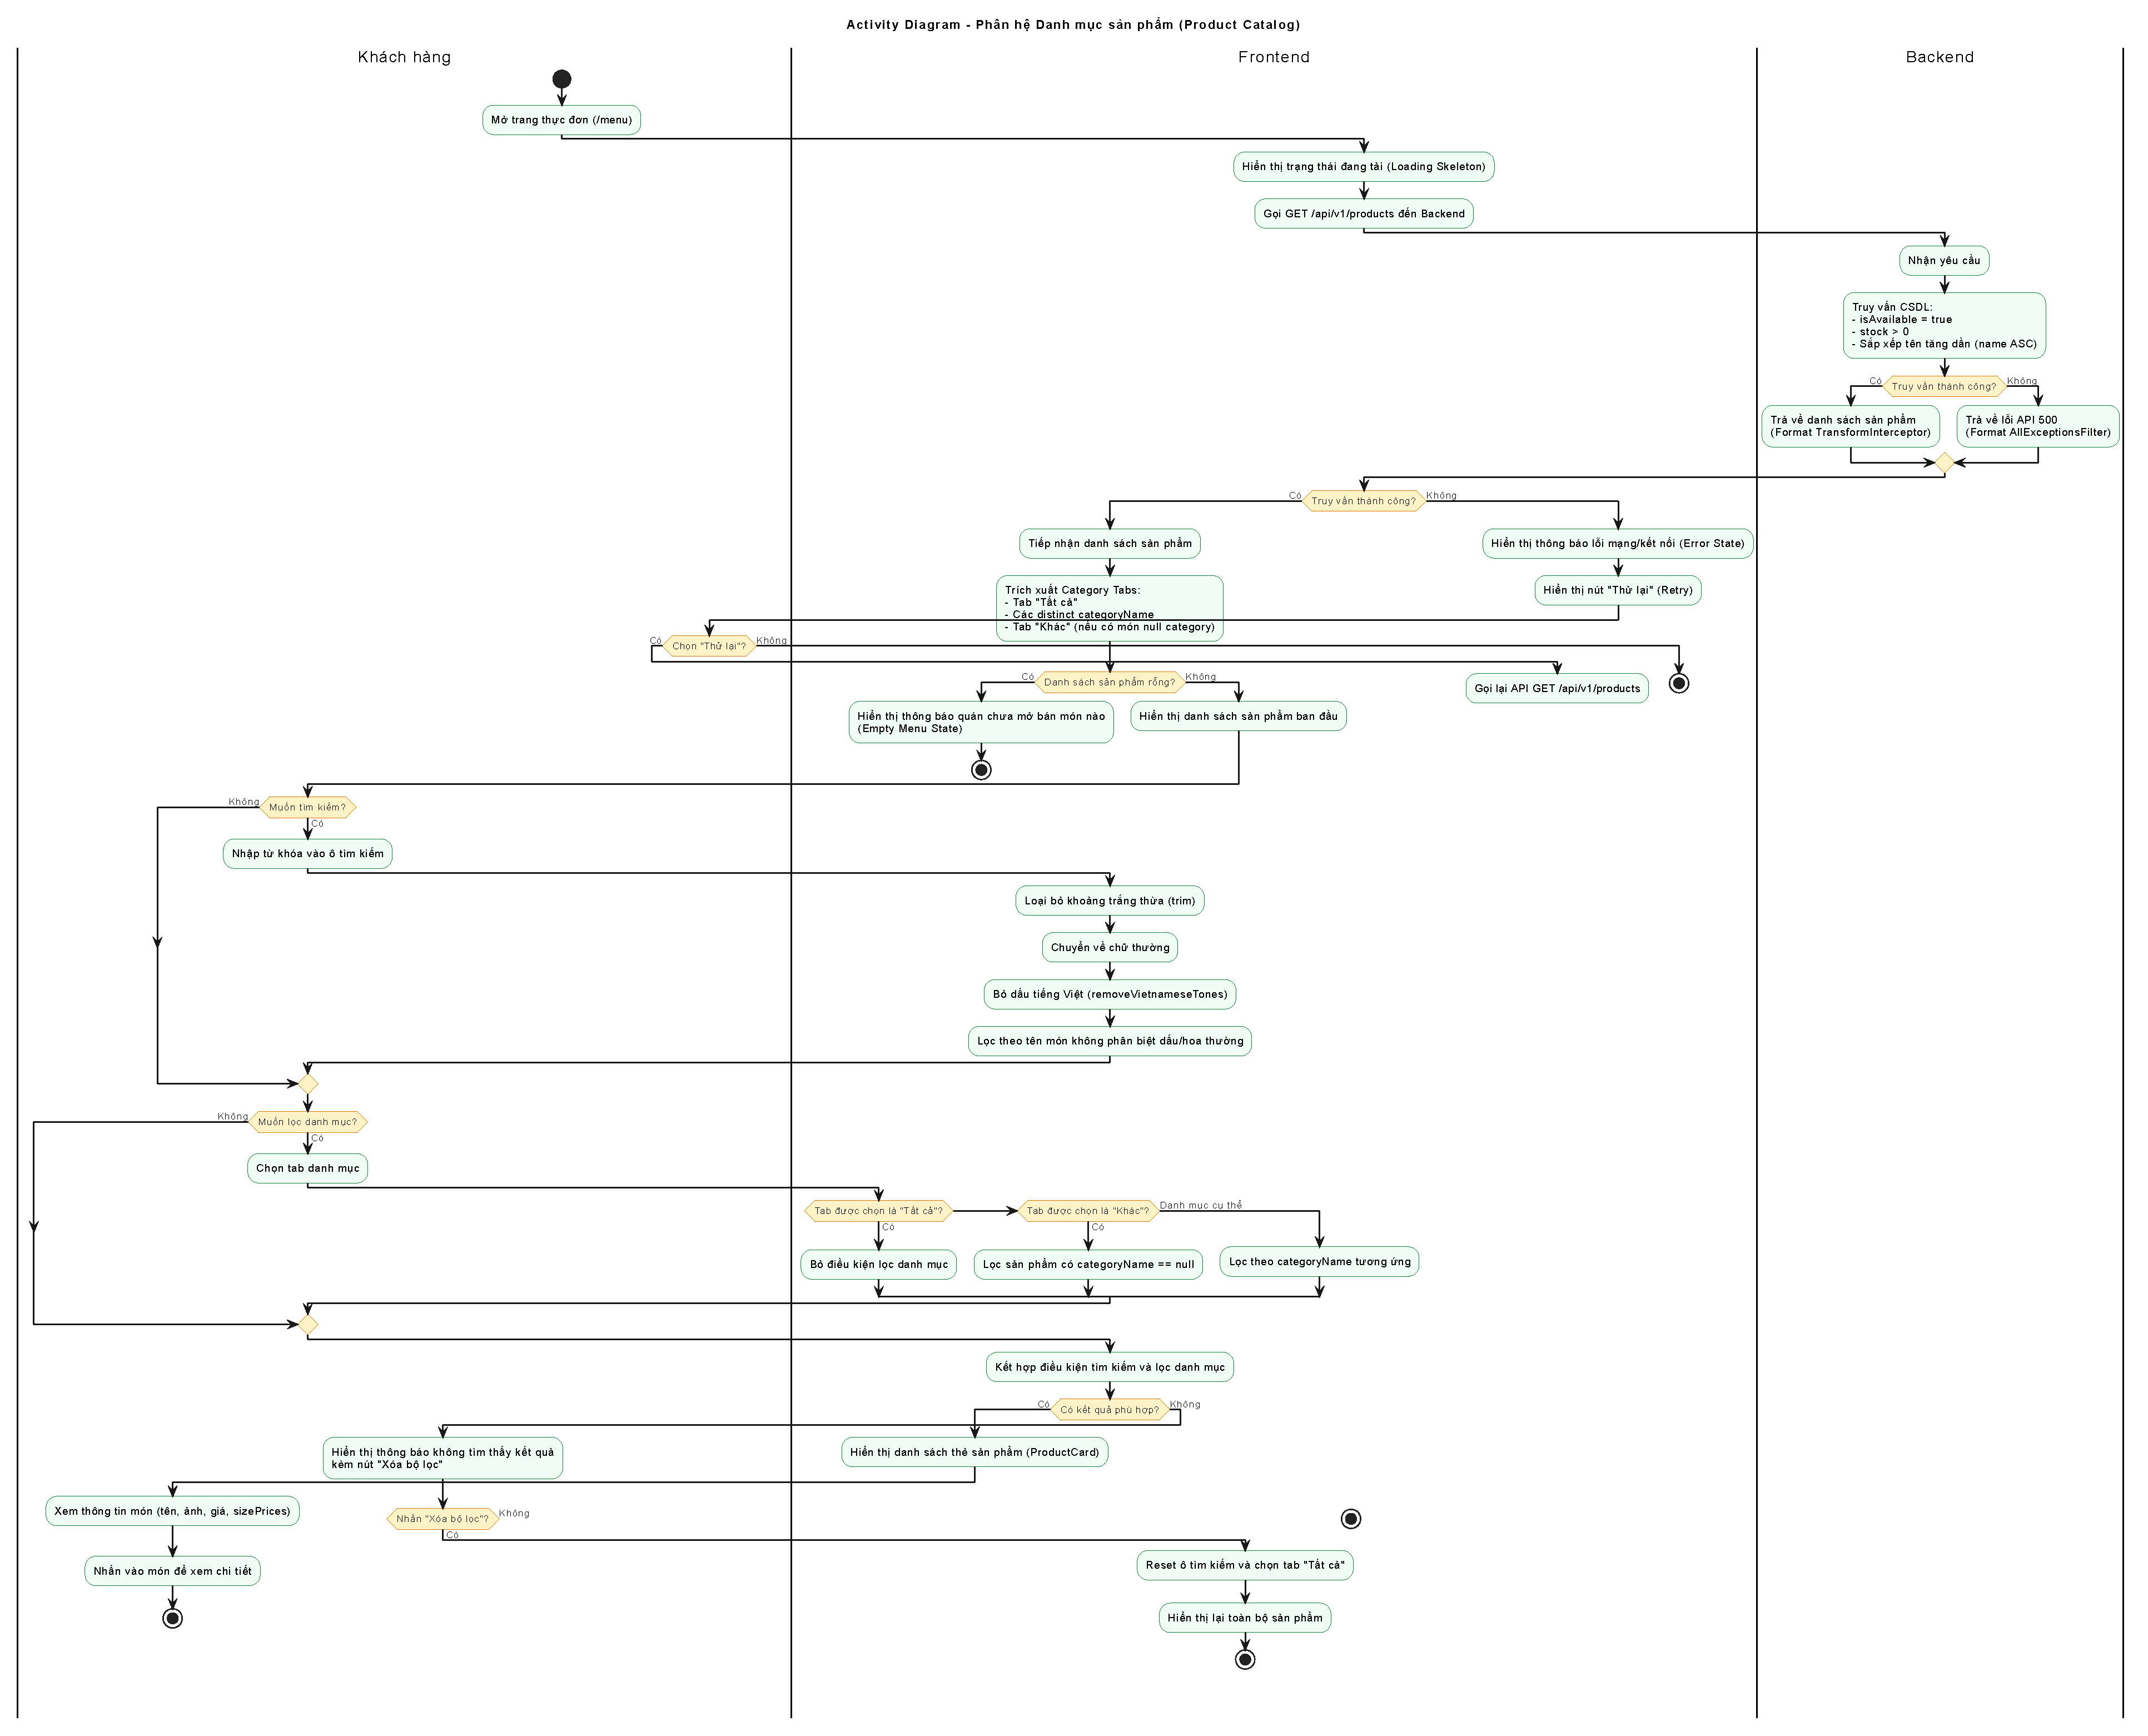
\includegraphics[width=\textwidth, height=0.98\textheight, keepaspectratio]{figures/activity-product-catalog.pdf}
    \caption{Sơ đồ Hoạt động - Phân hệ Danh mục Sản phẩm}
    \label{fig:activity-product-catalog}
\end{figure}

\clearpage
\subsection{Sơ đồ Tuần tự (Sequence Diagram)}
Sơ đồ Tuần tự phản ánh quá trình truy vấn danh mục và sản phẩm từ Frontend đến Backend Controller, Service và Prisma tại Hình~\ref{fig:sequence-product-catalog}.

\begin{figure}[H]
    \centering
    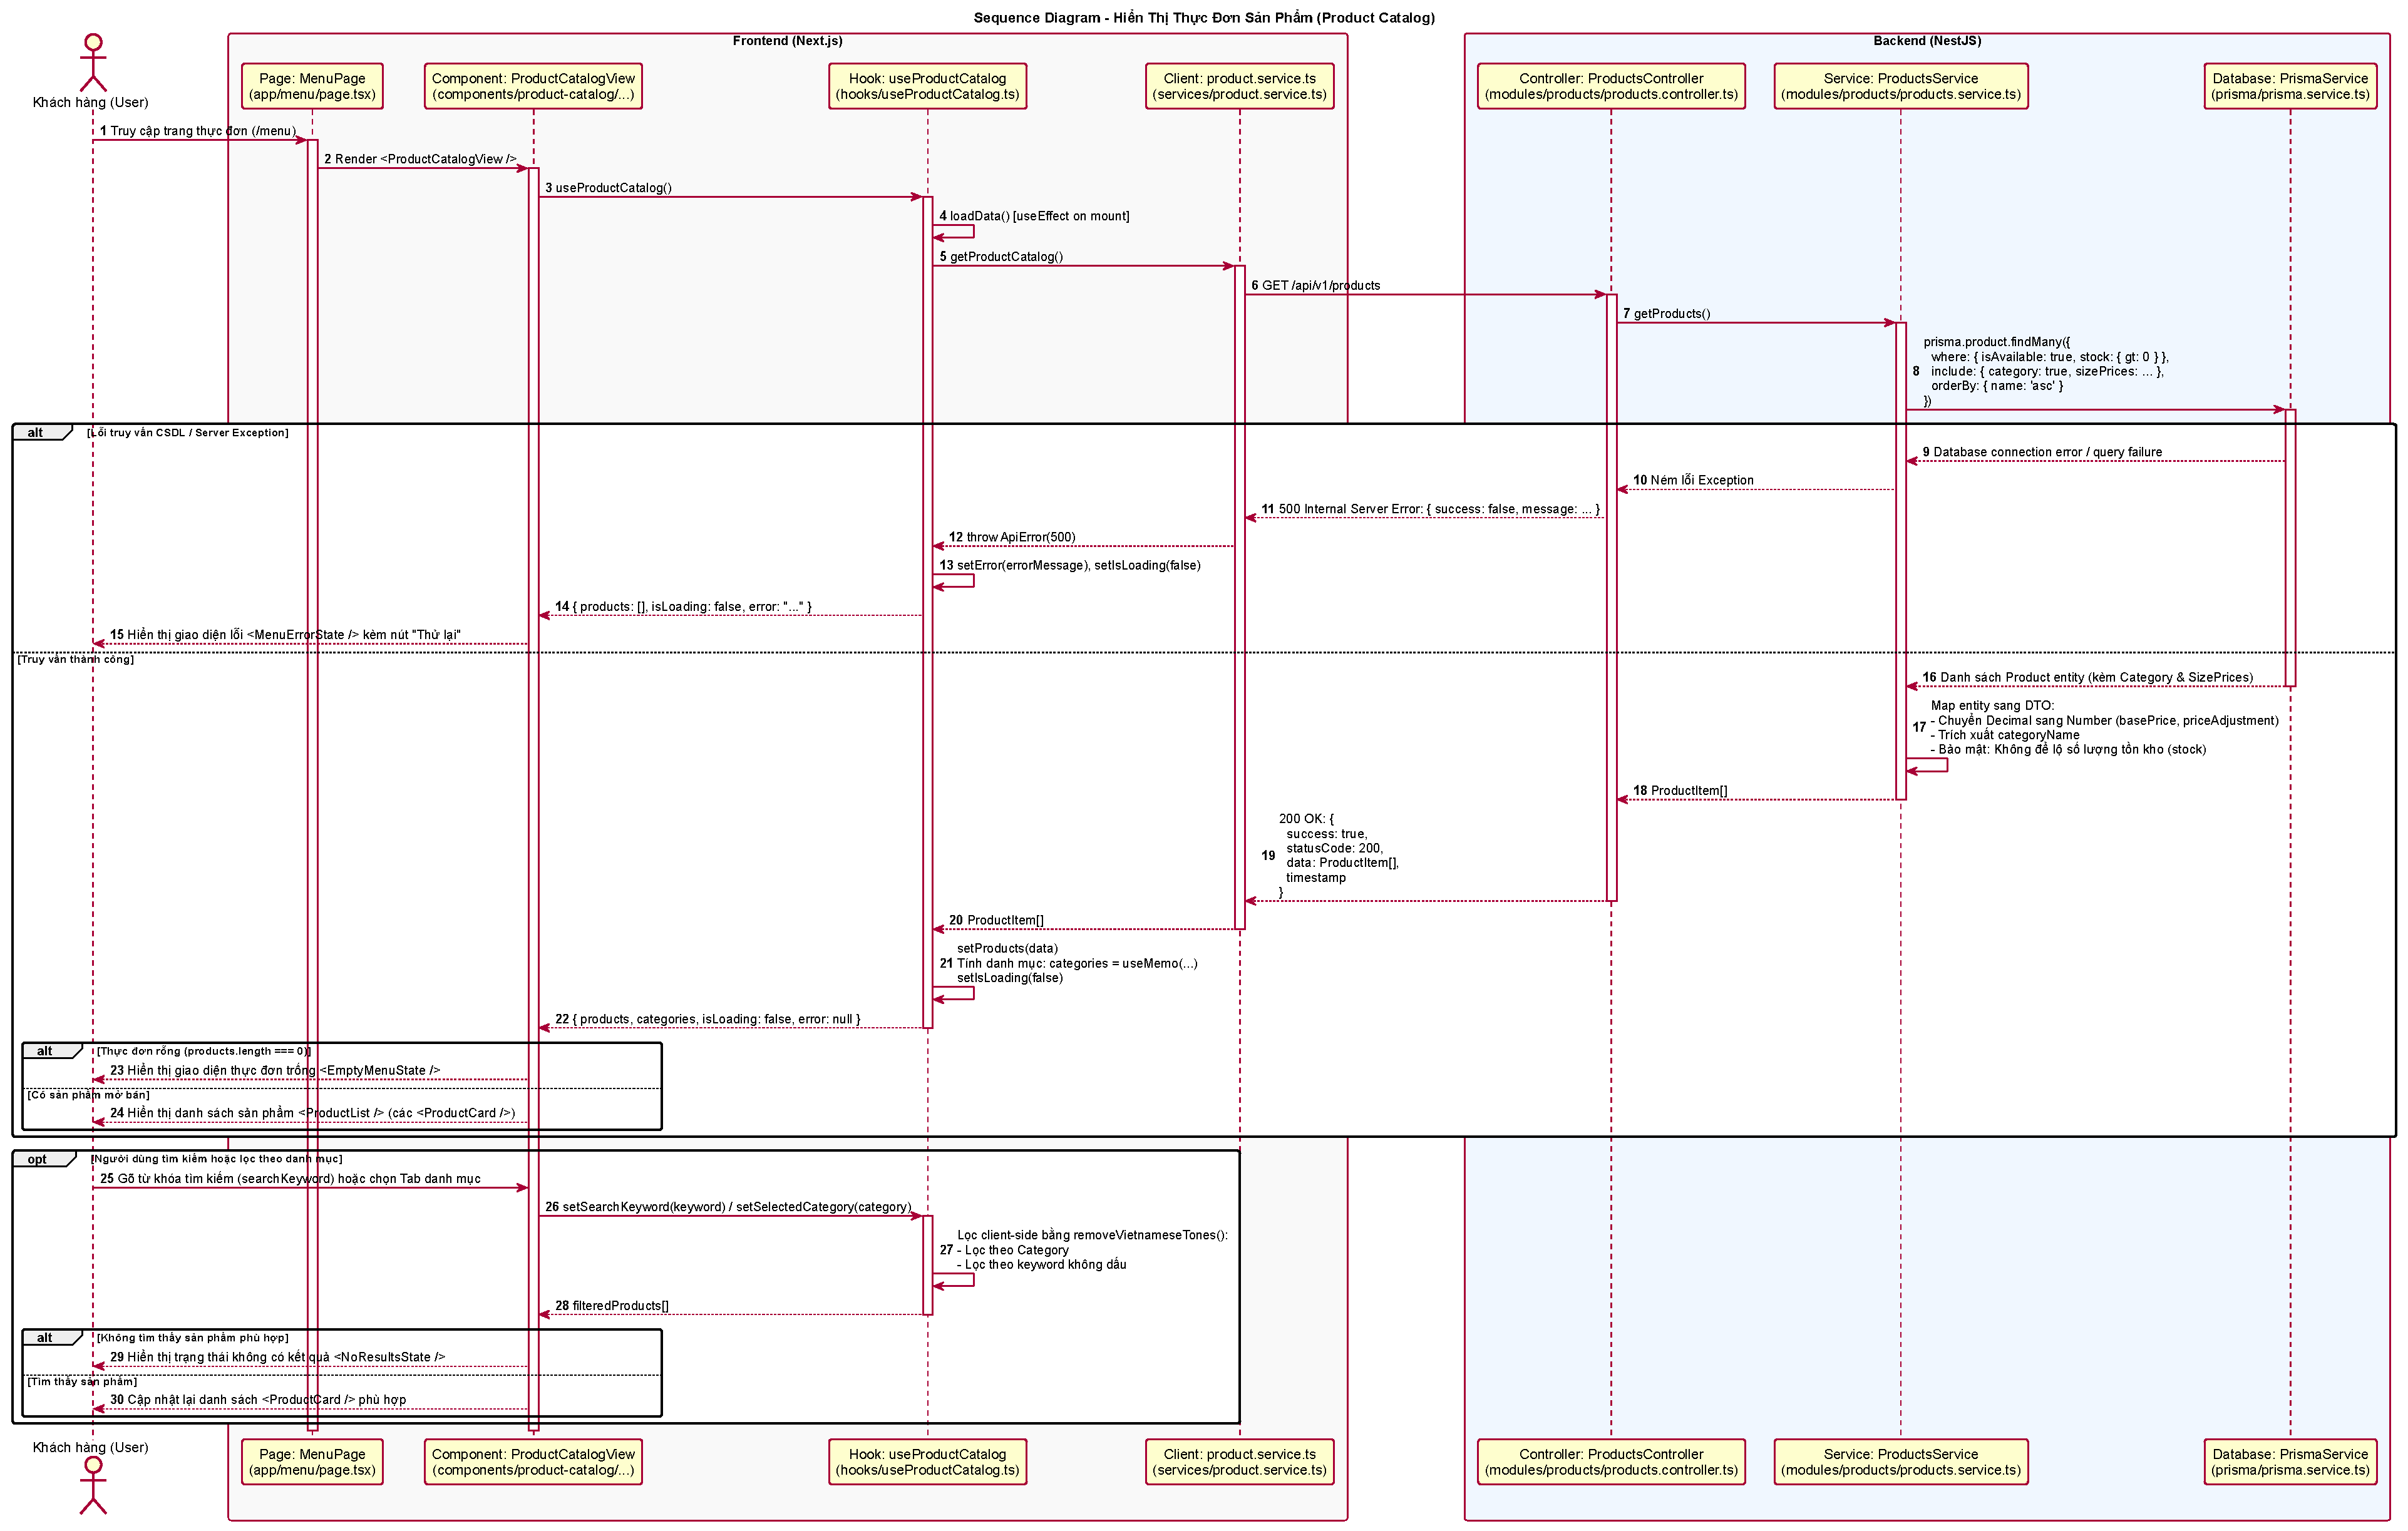
\includegraphics[width=\textwidth, height=0.80\textheight, keepaspectratio]{figures/sequence-product-catalog.pdf}
    \caption{Sơ đồ Tuần tự - Phân hệ Danh mục Sản phẩm}
    \label{fig:sequence-product-catalog}
\end{figure}

\clearpage
\subsection{Hợp đồng API (API Contract)}
\begin{table}[H]
\centering
\small
\caption{Danh mục API Endpoints - Phân hệ Danh mục Sản phẩm}
\label{tab:api-catalog}
\begin{tabularx}{\textwidth}{llp{4cm}X}
\toprule
\textbf{Phương thức} & \textbf{Endpoint} & \textbf{Tham số Query} & \textbf{Phản hồi chính} \\
\midrule
\texttt{GET} & \texttt{/api/v1/categories} & Không có & \texttt{200 OK}: Danh sách danh mục sắp xếp theo \texttt{displayOrder} tăng dần. \\
\texttt{GET} & \texttt{/api/v1/products} & \texttt{categoryId}, \texttt{search}, \texttt{availableOnly} & \texttt{200 OK}: Danh sách sản phẩm kèm thông tin giá cơ bản, hình ảnh và trạng thái khả dụng. \\
\bottomrule
\end{tabularx}
\end{table}

\subsection{Ánh xạ Cơ sở dữ liệu (Database Mapping)}
\begin{itemize}
    \item Truy vấn danh mục: \texttt{prisma.category.findMany(\{ orderBy: \{ displayOrder: 'asc' \} \})}.
    \item Truy vấn sản phẩm: \texttt{prisma.product.findMany(\{ where: \{ ...filter \}, include: \{ sizePrices: true, category: true \} \})}.
    \item Dữ liệu seed chuẩn gồm 2 danh mục chính ("Cà phê" - 6 món, "Trà" - 4 món), tổng cộng 10 sản phẩm mẫu được nạp vào bảng \texttt{categories} và \texttt{products}.
\end{itemize}

\subsection{Kịch bản Kiểm thử (Test Cases)}
\begin{table}[H]
\centering
\small
\caption{Tóm lược các Ca kiểm thử tiêu biểu - Phân hệ Danh mục}
\label{tab:tc-catalog}
\begin{tabularx}{\textwidth}{llp{2.6cm}p{3cm}Xc}
\toprule
\textbf{Mã TC} & \textbf{Loại} & \textbf{Tiền điều kiện} & \textbf{Endpoint / Màn hình} & \textbf{Kết quả mong đợi} & \textbf{Trạng thái} \\
\midrule
\texttt{TC-CAT-API-01} & Hợp lệ & DB có 2 danh mục & \texttt{GET /categories} & Trả về đủ 2 danh mục "Cà phê", "Trà" & Chưa chạy \\
\texttt{TC-CAT-API-02} & Hợp lệ & DB có 10 sản phẩm & \texttt{GET /products} & Trả về danh sách 10 món kèm \texttt{basePrice} & Chưa chạy \\
\texttt{TC-CAT-UI-01} & Giao diện & Trang \texttt{/products} & Thực đơn chính & Hiển thị tab "Tất cả", "Cà phê", "Trà" & Chưa chạy \\
\texttt{TC-CAT-UI-07} & Giao diện & Chọn tab "Cà phê" & Lọc danh mục & Hiển thị đúng 6 món cà phê từ seed data & Chưa chạy \\
\bottomrule
\end{tabularx}
\end{table}

\subsection{Giao diện Người dùng}
\begin{figure}[H]
    \centering
    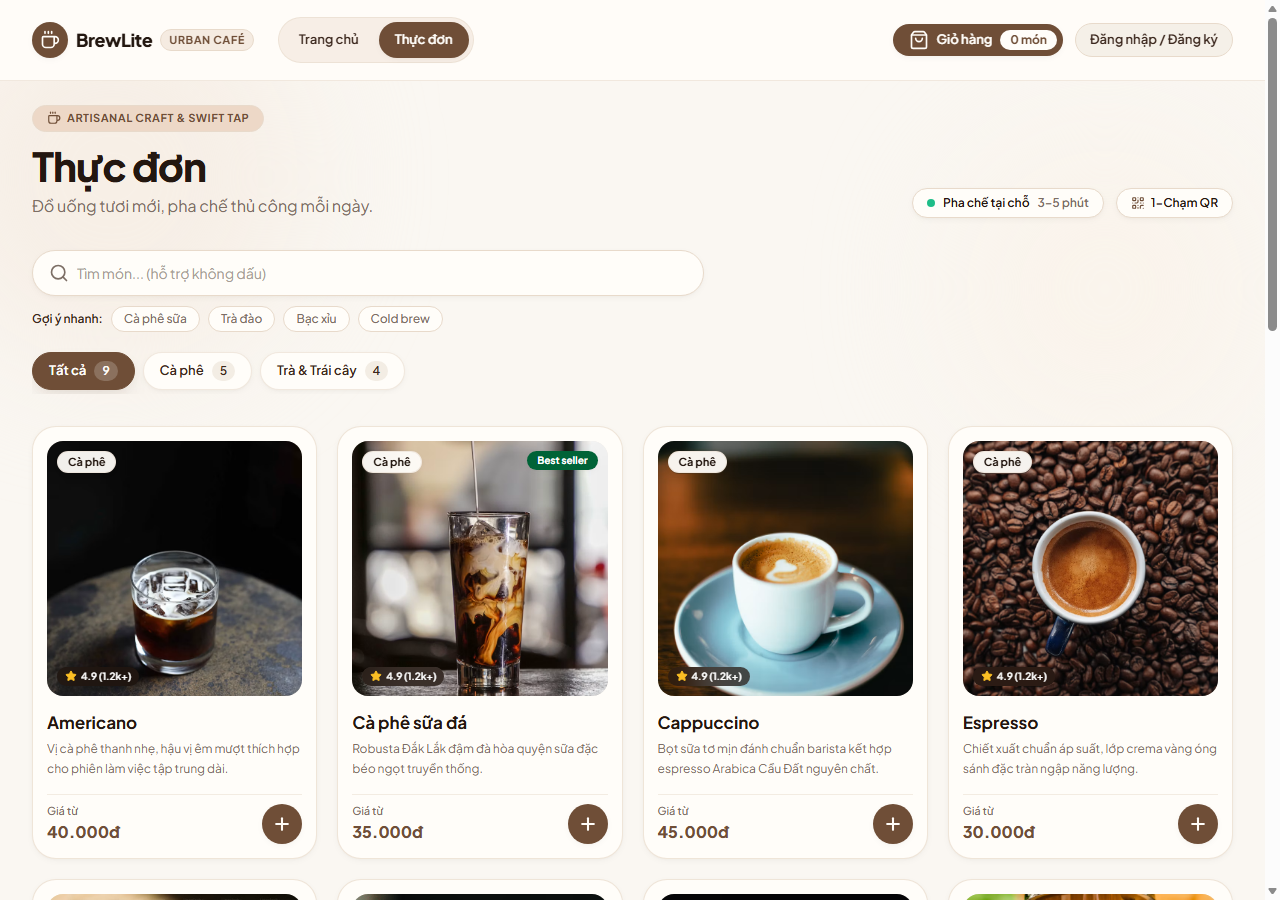
\includegraphics[width=0.92\textwidth]{figures/ui-catalog.png}
    \caption{Giao diện Thực đơn sản phẩm và Bộ lọc danh mục BrewLite}
    \label{fig:ui-catalog}
\end{figure}
